%-----------------------------------------------------------------------------%
\chapter{\babEmpat}
%-----------------------------------------------------------------------------%
Bab ini membahas tentang implementasi perangkat \textit{gateway}. Hal ini meliputi persiapan alat, implementasi \textit{gateway}, dan implementasi halaman kontrol.

\section{Persiapan Alat}
Alat yang digunakan pada tugas akhir ini adalah sebuah Raspberry Pi, sebuah \textit{shield} bernama RaspBee, dan WiFi dongle dengan merek Tenda. Tipe Raspberry Pi yang digunakan untuk tugas akhir ini adalah Raspberry Pi Model B dengan spesifikasi \textit{processor} 700 MHz \textit{single core}, 512 MB RAM, dan sebuah \textit{micro SD} 8GB. Sistem operasi yang digunakan adalah Raspbian, sebuah modifikasi distro linux Debian yang dibuat untuk Raspberry Pi. Gambar \ref{fig:raspberry} menunjukkan foto dari perangkat Raspberry Pi yang digunakan.

\begin{figure}
	\centering
	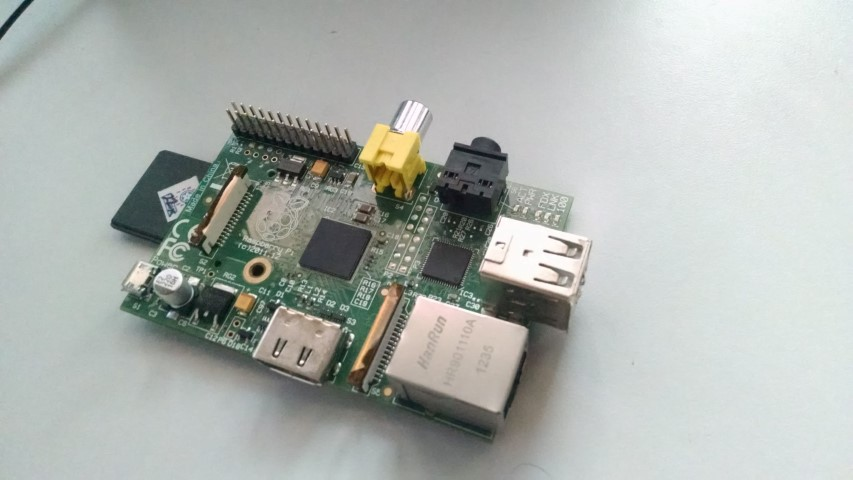
\includegraphics[width=.9\textwidth]{pics/raspberry.jpg}
	\caption{Raspberry Pi Model B}
	\label{fig:raspberry}
\end{figure}

Di dalam Raspberry Pi tersebut dipasang berbagai aplikasi dan \textit{tools} yang dibutuhkan untuk pengerjaan tugas akhir ini, seperti deCONZ, apache \textit{server}, dan MySQL \textit{server}. Berbagai aplikasi dan berkas yang diperlukan diatur agar otomatis berjalan ketika Raspberry Pi dinyalakan. Perangkat lain yang digunakan untuk menghubungkan Raspberry Pi dengan jaringan lampu ZigBee adalah RaspBee. RaspBee dapat dihubungkan dengan Raspberry Pi melalui port GPIO yang tersedia pada Raspberry Pi. Gambar \ref{fig:raspbee} menunjukkan foto perangkat RaspBee yang digunakan, dan gambar \ref{fig:raspbeeraspberry} menunjukkan foto perangkat RaspBee ketika dipasang pada Raspberry Pi yang digunakan.

\begin{figure}
	\centering
	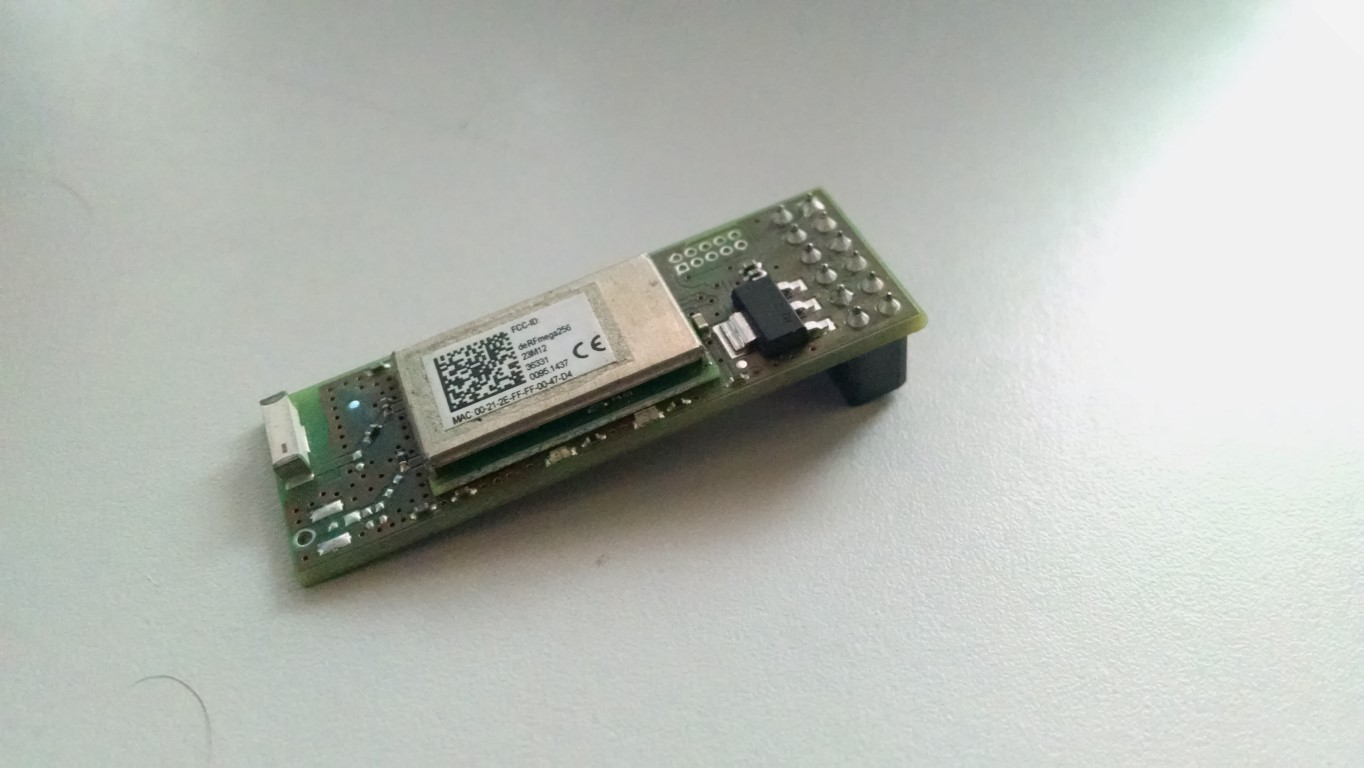
\includegraphics[width=.9\textwidth]{pics/raspbee.jpg}
	\caption{Perangkat RaspBee yang digunakan}
	\label{fig:raspbee}
\end{figure}
\begin{figure}
	\centering
	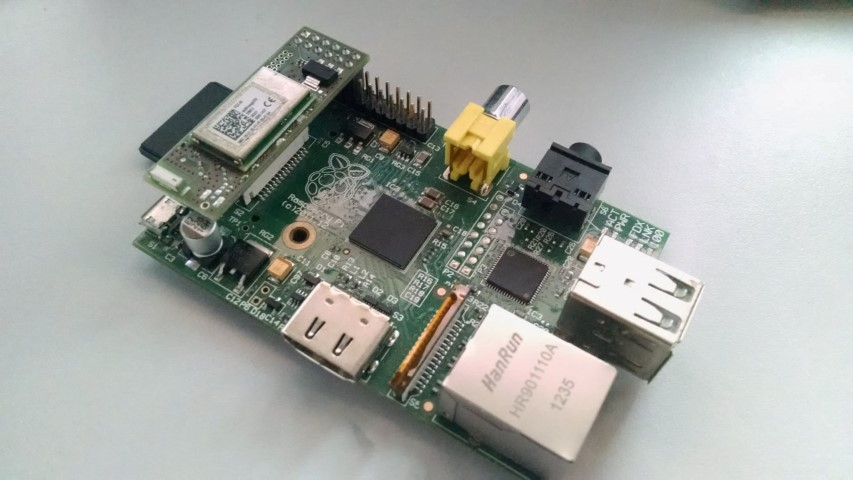
\includegraphics[width=.9\textwidth]{pics/raspberry+raspbee.jpg}
	\caption{Perangkat RaspBee ketika dipasang pada Raspberry Pi}
	\label{fig:raspbeeraspberry}
\end{figure}

Selain Raspberry Pi dan RaspBee, dibutuhkan juga sebuah modul WiFi agar perangkat \textit{gateway} bisa menjadi sebuah \textit{access point} dan bisa terhubung ke \textit{access point} lain. Hal ini dibutuhkan agar pengguna bisa terhubung ke perangkat \textit{gateway} dan perangkat gateway bisa terhubung ke internet. Untuk ini, diperlukan sebuah modul WiFi yang bisa berperan sebagai \textit{access point} dan di saat yang sama melakukan hubungan dengan \textit{access point} lain. Karena keterbatasan perangkat yang ada, dalam tugas akhir ini akan digunakan dua buah WiFi \textit{dongle} dengan merek Tenda untuk menjadi sebuah modul WiFi yang diinginkan. Gambar \ref{fig:tenda} menunjukkan foto kedua WiFi \textit{dongle} yang digunakan pada tugas akhir ini.
\begin{figure}
	\centering
	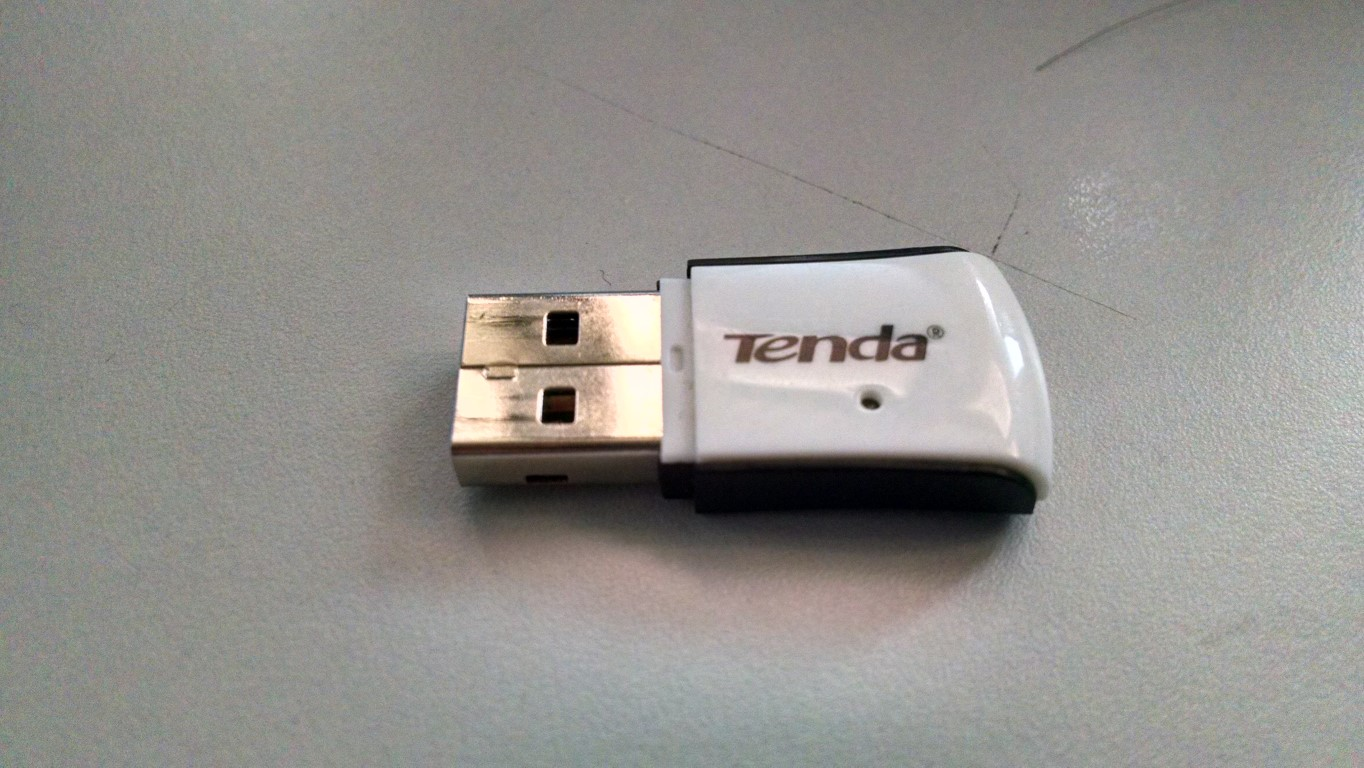
\includegraphics[width=.9\textwidth]{pics/tenda.jpg}
	\caption{WiFi \textit{dongle} yang digunakan}
	\label{fig:tenda}
\end{figure}

\section{Implementasi \textit{Gateway}}
Implementasi \textit{gateway} pada tugas akhir ini adalah implementasi terkait pengiriman data ke \plat~atau menerima data dari \plat~dan disampaikan ke lampu yang dituju. Hal ini meliputi implementasi MQTT \textit{client} dan translasi pesan MQTT ke perintah REST untuk disampaikan ke deCONZ.

\subsection{Implementasi MQTT \textit{Client}}
Pembuatan MQTT \textit{client} pada tugas akhir ini dilakukan dengan menggunakan \textit{library} Paho yang dibuat oleh Eclipse, dan dengan memodifikasi kode yang dibuat oleh Fauziah Rahmah dalam tugas akhirnya \cite{SkripsiFarah}. Selain itu, digunakan juga \textit{library} JDBC yang dibuat oleh Oracle untuk bisa terhubung dengan \textit{database} MySQL.

Langkah pertama yang dilakukan saat program dijalankan adalah membuat sebuah objek \textit{gateway} sekaligus menjalankan sebuah \textit{timer} untuk menjalankan sebuah fungsi di dalam objek tersebut setiap sepuluh detik. Hal ini dilakukan karena terdapat sebuah tugas yang harus dilakukan setiap suatu jangka waktu tertentu secara terus menerus, yaitu mengambil informasi mengenai lampu dan mengirimkannya ke \plat. Berikut merupakan potongan kode untuk membuat objek \textit{gateway} sekaligus menjalankan \textit{timer}.

\begin{lstlisting}[language=Java,label=code:timer,caption=Membuat objek \textit{gateway}]
Timer timer = new Timer();
timer.schedule(new Gateway(), 0, 10000);
\end{lstlisting}

Ketika objek \textit{gateway} dibuat, hal yang pertama dilakukan adalah mengambil id pengguna yang tersimpan di \textit{database} lokal perangkat \textit{gateway}. Setelah mendapat id pengguna, kemudian dibuat objek \textit{client} MQTT yang berperan sebagai \textit{publisher} dan \textit{subscriber}. Ketika membuat objek \textit{client}, parameter yang dibutuhkan adalah URI yang memberitahukan alamat dari \textit{broker}. Dalam tugas akhir ini, alamat \textit{broker} sekaligus merupakan alamat \plat~, yaitu 128.199.236.53, dan \textit{port default} yang digunakan oleh MQTT adalah 1883. Berikut merupakan potongan kode untuk membuat objek \textit{client} MQTT.

 \begin{lstlisting}[language=Java,label=code:client,caption=Membuat objek \textit{client} MQTT]
 //mengambil user id
 this.userID = getUserId();
 try {
// membuat client sebagai publisher
clientPub = new MqttClient("tcp://128.199.236.53:1883", "Publisher");
System.out.println("Publisher created");
// membuat client sebagai subscriber
clientSub = new MqttClient("tcp://128.199.236.53:1883", "Subscriber");
System.out.println("Subscriber created");
 \end{lstlisting}
 
 Setelah objek \textit{client} dibuat, \textit{client} tersebut kemudian perlu dihubungkan dengan \textit{broker}. Ketika dihubungkan dengan \textit{broker}, \textit{client} yang berperan sebagai \textit{subscriber} akan sekaligus melakukan proses \textit{subscribe} ke sebuah topik tertentu. Topik ini harus spesifik hanya untuk satu pengguna, namun dapat menerima semua pesan yang berkaitan dengan pengguna tersebut. Oleh karena itu, digunakanlah \textit{single level wildcard} untuk kebutuhan tersebut. Berikut adalah potongan kode untuk menghubungkan \textit{client} dengan \textit{broker}.
 
 \begin{lstlisting}[language=Java,label=code:timer,caption=Menghubungkan \textit{client} dengan \textit{broker}]
connectMosquitto(clientSub);
connectMosquitto(clientPub);
...
c.connect();
c.setCallback(this);
if(c.getClientId().equalsIgnoreCase("Subscriber")){
// client diatur agar bisa menerima pesan dari broker
c.setCallback(Gateway.this);
String topik = "sot/g/"+userID+"/+/+/+/ctl";
System.out.println(topik);
c.subscribe(topik);
System.out.println("Subscriber connected");
 \end{lstlisting}

Seperti yang telah dijelaskan sebelumnya, bahwa setiap sepuluh detik, \textit{gateway} akan mengirimkan informasi ke \textit{broker} mengenai kondisi lampu yang terhubung. Untuk melakukan hal ini, pertama \textit{gateway} perlu melihat di \textit{database} lokal mengenai informasi lampu yang terhubung dan informasi apa saja yang ingin dibagikan ke \plat. Setelah itu, \textit{client} yang berperan sebagai \textit{publisher} akan melakukan \textit{publishing} informasi-informasi tersebut. Proses \textit{publishing} dilakukan dengan mekanisme yang dijelaskan sebelumnya, yaitu satu topik untuk setiap atribut pada setiap lampu. Berikut adalah potongan kode yang melakukan \textit{publishing} tersebut.

\lstinputlisting[language=Java,label=code:timer,caption=\textit{Publishing} yang dilakukan setiap sepuluh detik]{code/run.java}

Setiap kali \textit{broker} mengirim pesan ke \textit{gateway}, sebuah \textit{method} pada objek \textit{gateway}, yaitu \textit{method} \texttt{messageArrived} akan dipanggil. \textit{Method} ini merupakan \textit{method} yang di\textit{override} dari \textit{interface} \texttt{MqttCallback}. \textit{Method} ini memiliki dua buah parameter, yaitu topik dengan tipe data \texttt{String} dan isi pesan dengan tipe data \texttt{MqttMessage}. Pesan yang diterima kemudian perlu diubah menjadi \texttt{String} agar bisa diolah dengan mudah. Kemudian, topik dan isi pesan dikirimkan ke \textit{method} \texttt{checkCommand} yang fungsinya akan dijelaskan pada bagian selanjutnya. Berikut merupakan potongan kode \textit{method} \texttt{messageArrived}.

\begin{lstlisting}[language=Java,label=code:timer,caption=\textit{Method} messageArrived]
@Override
public void messageArrived(String topic, MqttMessage msg){
	System.out.println("Topic : " + topic + ", message : " + msg);
	String command = msg.toString();
	// mengecek isi pesan dari broker
	checkCommand(topic, command);
}
\end{lstlisting}

\subsection{Translasi Pesan MQTT ke Pesan REST}
Seperti yang dijelaskan sebelumnya, bahwa perlu dilakukan translasi atau perubahan bentuk perintah, dari yang berupa topik dan pesan MQTT, menjadi sebuah perintah untuk mengeksekusi API REST yang disediakan oleh deCONZ. Perintah yang diterima dan diteruskan ke deCONZ dibatasi hanya sebatas atribut apa saja yang diperbolehkan oleh pengguna untuk dikontrol dari \plat. Proses ini dilakukan dalam \textit{method} \texttt{checkCommand} yang telah disebutkan dalam bagian sebelumnya. Pada \textit{method} inilah dilakukan pengolahan topik dan pesan dari \textit{broker} menjadi perintah REST.

Informasi yang disampaikan melalui topik adalah id perangkat atau lampu, dan atribut apa yang ingin di kontrol. Sedangkan untuk isi pesan, hanya berisi nilai baru dari atribut yang diinginkan. Id yang terdapat di dalam topik masih merupakan id yang disimpan oleh \textit{things management}, sehingga perlu diubah ke id lokal yang disimpan di dalam \textit{database}. Untuk mendapatkan id lokal, telah dibuat method bernama \texttt{getLocalId} yang menerima parameter id dari \textit{things management} dan mengembalikan id lokal yang tersimpan di \textit{database}. Selain itu, perlu diketahui juga apakah id yang dituju adalah sebuah lampu atau \textit{group}. Setelah mendapatkan id lokal dan tipe dari id yang dituju, selanjutnya dipanggil fungsi API REST yang disediakan oleh deCONZ. Potongan kode berikut menampilkan isi dari \textit{method} \texttt{checkCommand}.

\lstinputlisting[language=Java,label=code:timer,caption=\textit{Method} checkCommand]{code/checkCommand.java}

\section{Implementasi Halaman Kontrol Lampu}
Pengguna juga dapat melakukan kontrol terhadap lampu yang terhubung dengan langsung melalui perangkat \textit{gateway} atau tanpa harus terhubung ke internet. Untuk memenuhi hal ini, telah dibuat sebuah aplikasi berbasis web yang dijalankan di perangkat \textit{gateway} secara lokal. Aplikasi ini diimplementasikan menggunakan bahasa pemrograman PHP dan berjalan di atas \textit{server} Apache. Melalui aplikasi ini, pengguna dapat melakukan berbagai hal, sepert menghidupkan dan mematikan lampu, mengubah \textit{brightness}, mengubah \textit{hue}, dan mengubah \textit{saturation}. Pengguna juga dapat membuat \textit{group} yang terdiri dari lampu-lampu yang dimilikinya. Pengguna kemudian dapat melakukan \textit{log in} menggunakan akun \plat~yang dimilikinya, dan kemudian dapat mendaftarkan lampu dan \textit{group} yang ada ke \plat. Secara umum, terdapat dua halaman pada aplikasi web ini, yaitu halaman utama untuk mengontrol lampu dan \textit{group}, dan halaman untuk melakukan registrasi lampu atau \textit{group}.

\subsection{Halaman Utama Untuk Mengontrol Lampu}
Pada halaman ini, pengguna dapat melakukan beberapa hal, yaitu  melihat daftar lampu yang terhubung, menyalakan atau mematikan lampu, mengubah \textit{brightness} lampu, mengubah warna lampu, dan mengubah \textit{saturation} lampu. Pengguna juga dapat membuat \textit{group} lampu, dan terakhir pengguna dapat \textit{log in} menggunakan akun yang digunakan untuk mendaftar pada \plat.

\subsubsection{Melihat Daftar Lampu yang Terhubung}
Untuk bisa melihat daftar lampu yang terhubung, halaman ini akan menggunakan API REST yang disediakan oleh deCONZ. Untuk memanggil API REST yang disediakan deCONZ, digunakan fungsi \code{curl} yang sudah disediakan oleh PHP, dan \saya~membungkusnya menjadi sebuah fungsi bernama \texttt{kurl} yang menerima parameter \texttt{(String URI, String method, String data)}. Hasil dari pemanggilan API ini adalah sebuah objek JSON yang berisi daftar id lampu jika ada yang terhubung, atau objek kosong jika tidak ada lampu yang terhubung. Potongan kode berikut menampilkan kode untuk mengambil informasi daftar lampu yang terhubung.

\begin{lstlisting}[language=PHP,label=code:timer,caption=Mengambil informasi daftar lampu]
$output = kurl('localhost:8080/api/'.$apiKey."/lights","GET");
$listLampu = array();
if (!empty($output)) {
	$json_obj = json_decode($output);
	$id_lampu = [];
	foreach ($json_obj as $key => $value) {
	array_push($id_lampu, $key);
	}
\end{lstlisting}

\subsubsection{Mengubah Atribut Lampu}

Setelah mendapat info mengenai id lampu, kemudian API REST deCONZ digunakan lagi untuk mendapat informasi lebih detail mengenai setiap lampu. Informasi ini kemudian ditampilkan pada halaman utama aplikasi. Selain menampilkan informasi, halaman ini juga menampilkan beberapa elemen HTML untuk melakukan kontrol, seperti \textit{button} untuk menghidupkan atau mematikan lampu, \textit{range input} untuk mengubah \textit{brightness}, dan \textit{plugin} Javascript bernama JSColor untuk mengubah warna lampu. Masing-masing fungsi akan memanggil sebuah fungsi Javascript dan menggunakan fungsi AJAX untuk memanggil fungsi PHP yang bertugas menghubungi API REST deCONZ. Potongan kode berikut ini merupakan fungsi PHP yang dipanggil oleh halaman utama untuk memanggil API REST deCONZ. Fungsi ini dibuat agar bisa menerima permintaan kontrol untuk semua atribut.

\lstinputlisting[language=PHP,label=code:timer,caption=fungsi \texttt{setAttribute}]{code/setAttr.php}

\subsubsection{Membuat \textit{Group} Lampu}
Untuk membuat \textit{group}, digunakan API REST yang juga disediakan oleh deCONZ. Ketika memilih pilihan untuk membuat \textit{group} baru, pengguna akan diminta memasukkan nama \textit{group} dan memilih lampu yang mana saja yang akan dimasukkan ke dalam \textit{group} tersebut. Setelah itu, sebuah fungsi PHP akan dipanggil untuk mendaftarkan \textit{group} dengan informasi seperti yang diberikan oleh pengguna. Berikut adalah potongan kode untuk membuat \textit{group} baru.

\lstinputlisting[language=PHP,label=code:timer,caption=fungsi \texttt{createGroup}]{code/createGroup.php}

\subsubsection{\textit{Log In} Pengguna}
Untuk bisa mendaftarkan lampu dan group yang terhubung di perangkat \textit{gateway} ke \plat, diperlukan informasi id pengguna yang terdaftar di \plat. Oleh karena itu, pengguna diharuskan melakukan \textit{log in} sebelum mendaftarkan lampu atau \textit{group}. Dalam melakukan \textit{log in} ini, pengguna hanya perlu memasukkan email yang digunakan untuk mendaftar di \plat. Setelah \textit{log in} dan didapatkan id pengguna yang terdaftar di \plat, id ini akan disimpan di \textit{database} lokal untuk keperluan pendaftaran lampu dan \textit{group}. Informasi id ini juga akan digunakan oleh \textit{gateway} untuk melakukan proses \textit{subscribe} ke topik yang sesuai. Berikut ini adalah potongan kode untuk melakukan \textit{log in}.

\lstinputlisting[language=PHP,label=code:timer,caption=fungsi \texttt{createGroup}]{code/login.php}

\subsection{Implementasi Halaman Registrasi Lampu}
Pengguna dapat mendaftarkan lampu dan \textit{group} yang terhubung ke perangkat \textit{gateway} ke \plat. Karena kesamaan atribut yang dimiliki oleh lampu dan \textit{group}, ketika didaftarkan sebuah \textit{group} akan dianggap sebagai lampu. Saat mendaftarkan lampu atau \textit{group}, pengguna juga bisa sekaligus mendaftarkan atribut yang dimiliki oleh lampu atau \textit{group}. Atribut ini adalah \textit{On / Off}, \textit{brightness}, \textit{saturation}, dan \textit{hue}. Ketika mendaftarkan, pengguna diminta memilih hak akses bagi setiap atribut. Terdapat dua hak akses, yaitu hak untuk membagikan informasi terkait suatu atribut ke \plat, dan hak untuk memberikan hak kontrol suatu atribut dari \plat. Untuk mendaftarkan atribut, disediakan sebuah fungsi yang bernama \texttt{attrRegister} yang menerima parameter hak akses, nama, tipe, deskripsi, nilai minimal , dan nilai maksimal untuk suatu atribut. Berikut adalah potongan kode untuk mendaftarkan atribut.

\lstinputlisting[language=PHP,label=code:timer,caption=fungsi \texttt{attrRegister}]{code/attrRegister.php}

Setelah mendaftarkan lampu atau \textit{group} beserta atributnya, akan didapatkan informasi id perangkat dari \plat. Id ini kemudian disimpan di dalam \textit{database} lokal untuk digunakan oleh \textit{gateway}. Selain id, informasi mengenai atribut apa saja yang didaftarkan juga akan disimpan. Informasi ini digunakan oleh \textit{gateway} dalam menentukan atribut mana saja yang akan dilakukan proses \textit{subscribe} dan atribut mana yang akan dilakukan proses \textit{publishing}. Seluruh hal ini dilakukan dalam sebuah fungsi bernama \texttt{registerThings}. Berikut adalah potongan kode ketika mendaftarkan lampu atau \textit{group} serta ketika melakukan penyimpanan informasi ke \textit{database}.

\lstinputlisting[language=PHP,label=code:timer,caption=fungsi \texttt{registerThings}]{code/registerThings.php}

\section{Implementasi Perangkat Gateway}
Agar perangkat \textit{gateway} bisa berjalan seperti yang diinginkan, perlu dilakukan beberapa konfigurasi. Hal-hal yang perlu dikonfigurasi adalah pengaturan aplikasi yang berjalan ketika \textit{start up}, dan pengaturan agar perangkat \textit{gateway} bisa menjadi sebuah \textit{access point} dan dihubungkan ke \textit{access point} lain.

\subsection{Konfigurasi \textit{Start Up}}
Agar perangkat \textit{gateway} bisa berjalan tanpa perlu dilakukan secara manual oleh pengguna, perlu dibuat konfigurasi agar beberapa \textit{tools} atau aplikasi berjalan secara otomatis ketika perangkat menyala. \textit{Tools} yang diperlukan agar berjalan secara otomatis ketika perangkat menyala adalah deCONZ. deCONZ diperlukan karena seluruh operasi terkait lampu akan menggunakan API REST yang disediakan oleh deCONZ.

Untuk bisa berjalan, deCONZ memerlukan sebuah X \textit{server} yang sudah berjalan. Untuk menjalankan X \textit{server}, secara \textit{default} diperlukan pengguna untuk melakukan \textit{log in} menggunakan GUI. Untuk \textit{log in} menggunakan GUI pada Raspberry Pi, diperlukan sebuah layar eksternal atau penggunaan aplikasi lain. Karena perangkat \textit{gateway} ini ditargetkan agar bisa berjalan tanpa perangkat tambahan, maka perlu dilakukan konfigurasi agar perangkat secara otomatis menjalankan sebuah X \textit{server} ketika menyala, dan mengarahkan X \textit{server} tersebut ke sebuah tty, sehingga tidak diperlukan sebuah layar. Setelah berhasil menjalankan X \textit{server}, deCONZ secara otomatis dijalankan pada X \textit{server} yang telah berjalan. Potongan kode berikut merupakan konfigurasi yang dibutuhkan untuk melakukan tersebut.

\begin{lstlisting}[language=bash,caption=kode untuk menjalankan X \textit{server} dan memulai deCONZ]
#!/bin/bash

X :8 vt8 > /tmp/X8.log 2>&1 &
X_PID=$!

export DISPLAY=:8
deCONZ --auto-connect=1 --http-port=8080

kill $X_PID
\end{lstlisting}

Pada potongan kode diatas, dijalankan sebuah X \textit{server} dan diarahkan pada tty8. Kemudian, log dari X \textit{server} diarahkan ke \textit{file} X8.log. Setelah itu, dilakukan pengaturan agar deCONZ dijalankan pada X \textit{server} yang telah dijalankan sebelumnya. Kode ini disimpan pada suatu \textit{file}, yang kemudian akan dijalankan ketika \textit{start up}. Untuk menjalankan \textit{file} tersebut ketika \textit{start up}, perlu dilakukan modifikasi \textit{file} \texttt{rc.local} pada \textit{folder} \texttt{/etc}. Pada \textit{file} tersebut, ditambahkan baris \texttt{/root/deconz > /root/deconz.out 2> /root/deconz.err \&}. Baris tersebut berarti ketika \textit{file} dijalankan, keluaran dari aplikasi yang dijalankan akan ditaruh ke dalam \textit{file} \texttt{deconz.out} dan jika terdapat \textit{error} akan ditaruh ke dalam \textit{file} \texttt{deconz.err}.

\subsection{Konfigurasi \textit{Access Point}}
Ketika pertama kali perangkat \textit{gateway} dijalankan, perangkat ini akan berfungsi sebagai sebuah \textit{access point}. Dengan ini, pengguna kemudian bisa terhubung ke perangkat \textit{gateway} dengan menggunakan komputer atau \textit{smartphone} yang dimilikinya. Untuk bisa menjadikan perangkat ini sebagai \textit{access point}, dibutuhkan sebuah aplikasi dengan nama hostapd. Pada hostapd, dilakukan konfigurasi seperti pada potongan kode berikut.

\begin{lstlisting}[language=bash,caption=Konfigurasi hostapd]
interface=wlan0
ssid=[access_point_name]
hw_mode=g
channel=6
auth_algs=1
wmm_enabled=0
\end{lstlisting}

Setelah dilakukan konfigurasi diatas, hostapd dapat dijalankan dengan perintah \code{service hostapd start}. Untuk menjalankan hostpad secara otomatis setiap perangkat \textit{gateway} dinyalakan, digunakan perintah \code{update-rc.d hostapd enable}. Setelah terhubung, pengguna dapat memilih \textit{access point} lain yang berada di sekitarnya yang memiliki koneksi internet melalui suatu halaman web yang disediakan. Untuk melihat \textit{access point} apa saja yang berada di sekitar perangkat, dapat digunakan perintah \code{iwlist wlan1 scan | grep ESSID}. Setelah ditampilkan, pengguna kemudian dapat melakukan klik pada \textit{access point} yang dipilih. Perangkat \textit{gateway} kemudian akan terhubung dengan \textit{access point} yang dipilih. Potongan kode berikut menunjukkan implementasi untuk terhubung ke suatu \textit{access point}.

\begin{lstlisting}[language=php,caption=Kode untuk terhubung ke suatu \textit{access point}]
if (isset($_GET['id'])) {
	$id = $_GET['id'];
	$bash = "sudo iwconfig wlan1 essid ".$id;
	$output = shell_exec($bash);
	$bash = "sudo dhclient wlan1";
	$output = shell_exec($bash);
}
\end{lstlisting}
